\chapter{Mon premier chapitre}
\section{Introduction}
\lipsum[1-1]%genère un texte aléatoire
\section{Une section}

\subsection{Une première sous-section}
\lipsum[1-1]%genère un texte aléatoire
\subsection{Une deuxième sous-section}

Exemple de citation\cite{deffog}. Exemple de référence de la figure \ref{cloud}.
\begin{figure}[H]
	\centering
	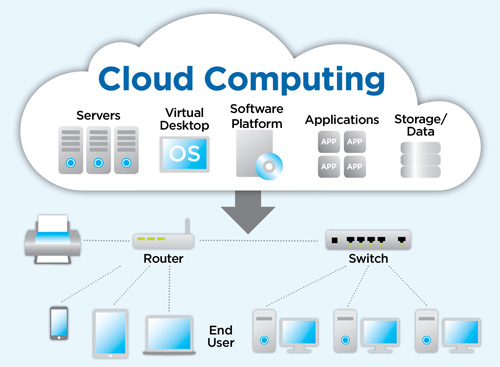
\includegraphics[scale=0.6]{figures/cloud-public.jpg}
	\caption{Architecture du Cloud}
	\label{cloud}
\end{figure}

\subsubsection{Sous-sous-sec1}
dsfsdf slkfj lsfj lkj lekj lzjeo fijzeif jzoiejf zoiej fozj efo
\subsubsection{Sous-sous-sec2}
Exemple de liste :

\begin{itemize}
	\item \textbf{Point 1}: azdpoakzd poakz poakz paokzd paokz 
	\item \textbf{Point 2}: csjc skjdc ksjd cksjc hskck s djc k
\end{itemize}
\subsection{Fog Computing}
azdazdazda a  jir iejrnf iejrnf ierjnf ierjn fiej ejnife
\section{Une autre section}
\lipsum[1-1] %genère un texte aléatoire